\twocolumn

\section{Additional Experiments and Details}\label{appendix:autoencoder}

In this section, we present additional experimental results that we did not include in the body of the paper for the sake of brevity. We still choose to provide them as additional substantiation of our arguments here. This section also contains additional details concerning the experiment setup for our examples where applicable. 

\subsection{Are Neural Networks Born with World Maps?}

The initial feature matrix \(X^{(n \times m)}\) is made up of \(n=4,217\) and \(m=10\) features.  We add a total of \(490\) random features to \(X\) to simulate the fact that not all features ingested by Llama-2 are necessarily correlated with geographical coordinates. That yields \(500\) features in total. The training subset contains \(3,374\) randomly drawn samples, while the remaining \(843\) are held out for testing. The single hidden layer of the untrained neural network has \(400\) neurons.

\subsection{LLMs for Economic Sentiment Prediction}

\subsubsection{Linear Probes}

Figures~\ref{fig-cpi} to~\ref{fig-ust-10} present average performance measures across folds for all indicators each time for the train and test set. We report the correlation between predictions and observed values (`cor'), the mean directional accuracy (`mda'), the mean squared error (`mse') and the root mean squared error (`rmse'). The model depth---as indicated by the number of the layer---increases along the horizontal axis.

Figures~\ref{fig-cpi-b} to~\ref{fig-ust-10-b} present the same performance measures, also for the baseline autoregressive model. Shaded areas show the variation across folds.

\subsubsection{Spark of Econonomic Understanding?}\label{appendix:sentences}

Below we present the 10 sentences in each category that were used to generate the probe predictions plotted in Figure~\ref{fig-attack}. In each case, the first 5 sentences were composed by ourselves. The following 5 sentences were generated using ChatGPT 3.5 using the following prompt followed by the examples in each category:

\begin{quote}
  ``I will share 5 example sentences below that sound a bit like they are about price deflation but are really about a deflation in the numbers of doves. Please generate an additional 25 sentences that are similar. Concatenate those sentences to the example string below, each time separating a sentence using a semicolon (just follow the same format I've used for the examples below). Please return only the concatenated sentences, including the original 5 examples. 

  Here are the examples:''
\end{quote}

This was followed up with the following prompt to generate additional sentences:

\begin{quote}
  ``Please generate X more sentences in the same manner and once again return them in the same format. Do not recycle sentences you have already generated, please.''
\end{quote}

All of the sentences were then passed through the linear probe for the CPI and sorted in ascending or descending order depending on the context (inflation or deflation). We then carefully inspected the list of sentences and manually selected 5 additional sentences to concatenate to the 5 sentences we composed ourselves.

\paragraph{Inflation/Prices}

The following sentences were used:

\begin{quote}
  Consumer prices are at all-time highs.;Inflation is expected to rise further.;The Fed is expected to raise interest rates to curb inflation.;Excessively loose monetary policy is the cause of the inflation.;It is essential to bring inflation back to target to avoid drifting into hyperinflation territory.;Inflation is becoming a global phenomenon, affecting economies across continents.;Inflation is reshaping the dynamics of international trade and competitiveness.;Inflationary woes are prompting governments to reassess fiscal policies and spending priorities.;Inflation is reshaping the landscape of economic indicators, challenging traditional forecasting models.;The technology sector is not immune to inflation, facing rising costs for materials and talent.
\end{quote}

\paragraph{Inflation/Birds}

The following sentences were used:

\begin{quote}
  The number of hawks is at all-time highs.;Their levels are expected to rise further.;The Federal Association of Birds is expected to raise barriers of entry for hawks to bring their numbers back down to the target level.;Excessively loose migration policy for hawks is the likely cause of their numbers being so far above target.;It is essential to bring the number of hawks back to target to avoid drifting into hyper-hawk territory.;The unprecedented rise in hawk figures requires a multi-pronged approach to wildlife management.;Environmental agencies are grappling with the task of addressing the inflationary hawk numbers through targeted interventions.;The burgeoning hawk figures highlight the need for adaptive strategies to manage and maintain a healthy avian community.;The unprecedented spike in hawk counts highlights the need for adaptive and sustainable wildlife management practices.;Conservationists advocate for proactive measures to prevent further inflation in hawk numbers, safeguarding the delicate balance of the avian ecosystem.
\end{quote}

\paragraph{Deflation/Prices}

The following sentences were used:

\begin{quote}
  Consumer prices are at all-time lows.;Inflation is expected to fall further.;The Fed is expected to lower interest rates to boost inflation.;Excessively tight monetary policy is the cause of deflationary pressures.;It is essential to bring inflation back to target to avoid drifting into deflation territory.;The risk of deflation may increase during periods of economic uncertainty.;Deflation can lead to a self-reinforcing cycle of falling prices and reduced economic activity.;The deflationary impact of reduced consumer spending can ripple through the entire economy.;Falling real estate prices can contribute to deflation by reducing household wealth and confidence.;The deflationary impact of falling commodity prices can have ripple effects throughout the global economy.
\end{quote}

\paragraph{Deflation/Birds}

The following sentences were used:

\begin{quote}
  The number of doves is at all-time lows.;Their levels are expected to fall further.;The Federal Association of Birds is expected to lower barriers of entry for doves to bring their numbers back up to the target level.;Excessively tight migration policy for doves is the likely cause of their numbers being so far below target.;Dovelation risks loom large as the number of doves continues to dwindle.;The number of doves is experiencing a significant decrease in recent years.;It is essential to bring the numbers of doves back to target to avoid drifting into dovelation territory.;A comprehensive strategy is needed to reverse the current dove population decline.;Experts warn that without swift intervention, we may witness a sustained decrease in dove numbers.
\end{quote}

We think that this sort of manual, LLM-aided adversarial attack against another LLM can potentially be scaled up to allow for rigorous testing, which we will turn to next.
 
% ---------- CPI ----------

\begin{figure*}

\centering{

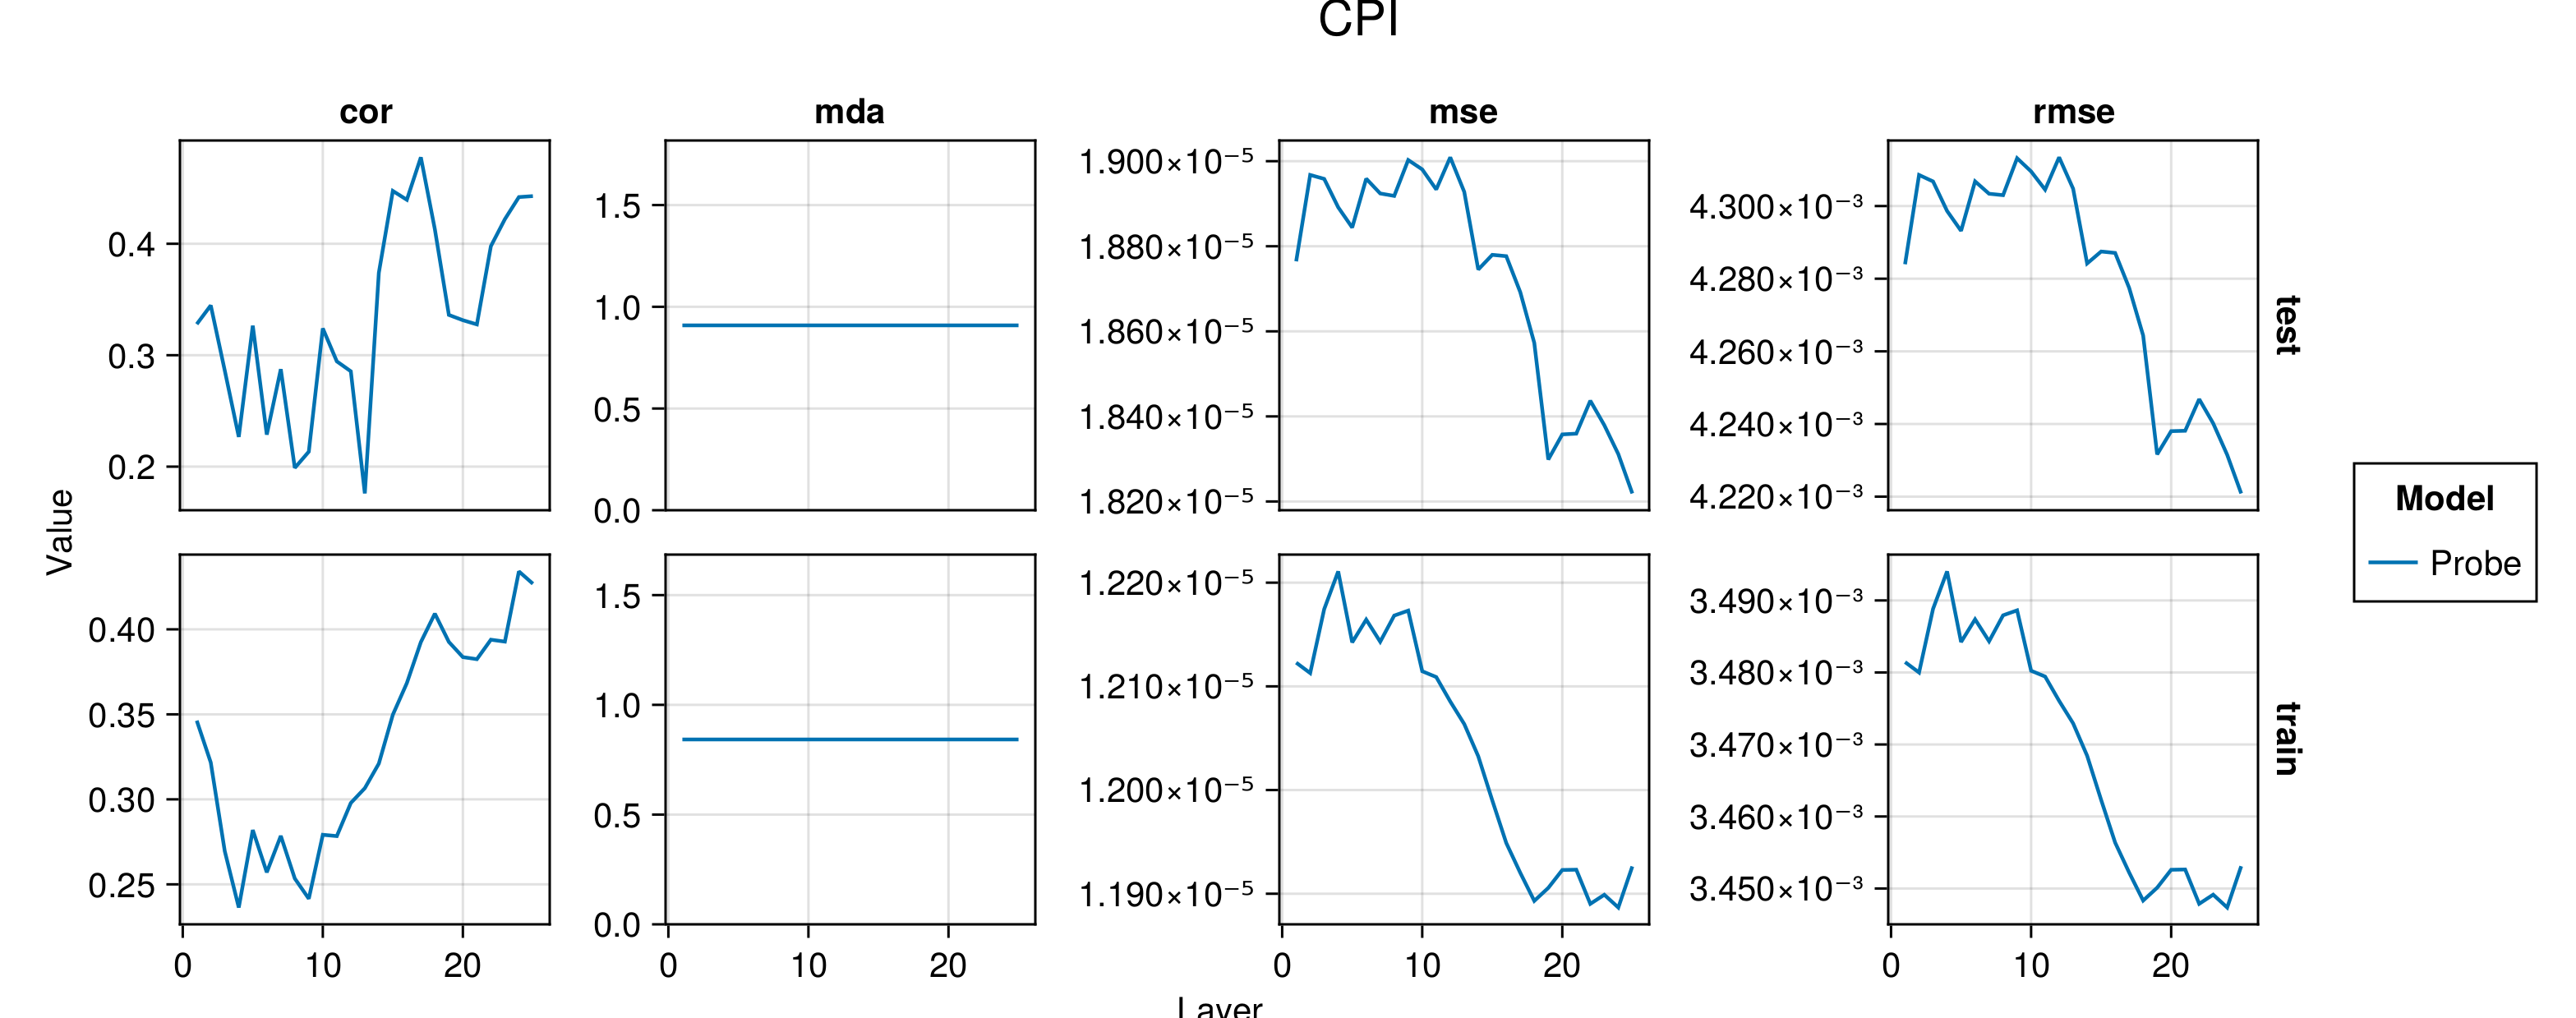
\includegraphics[width=1.0\textwidth]{results/figures/measures_probe_CPI (n_pc=128).png}

}

\caption{\label{fig-cpi}Average performance measures across folds plotted against model depth (number of layer) for the CPI for the train and test set.}

\end{figure*}%



% ---------- PPI ----------

\begin{figure*}

\centering{

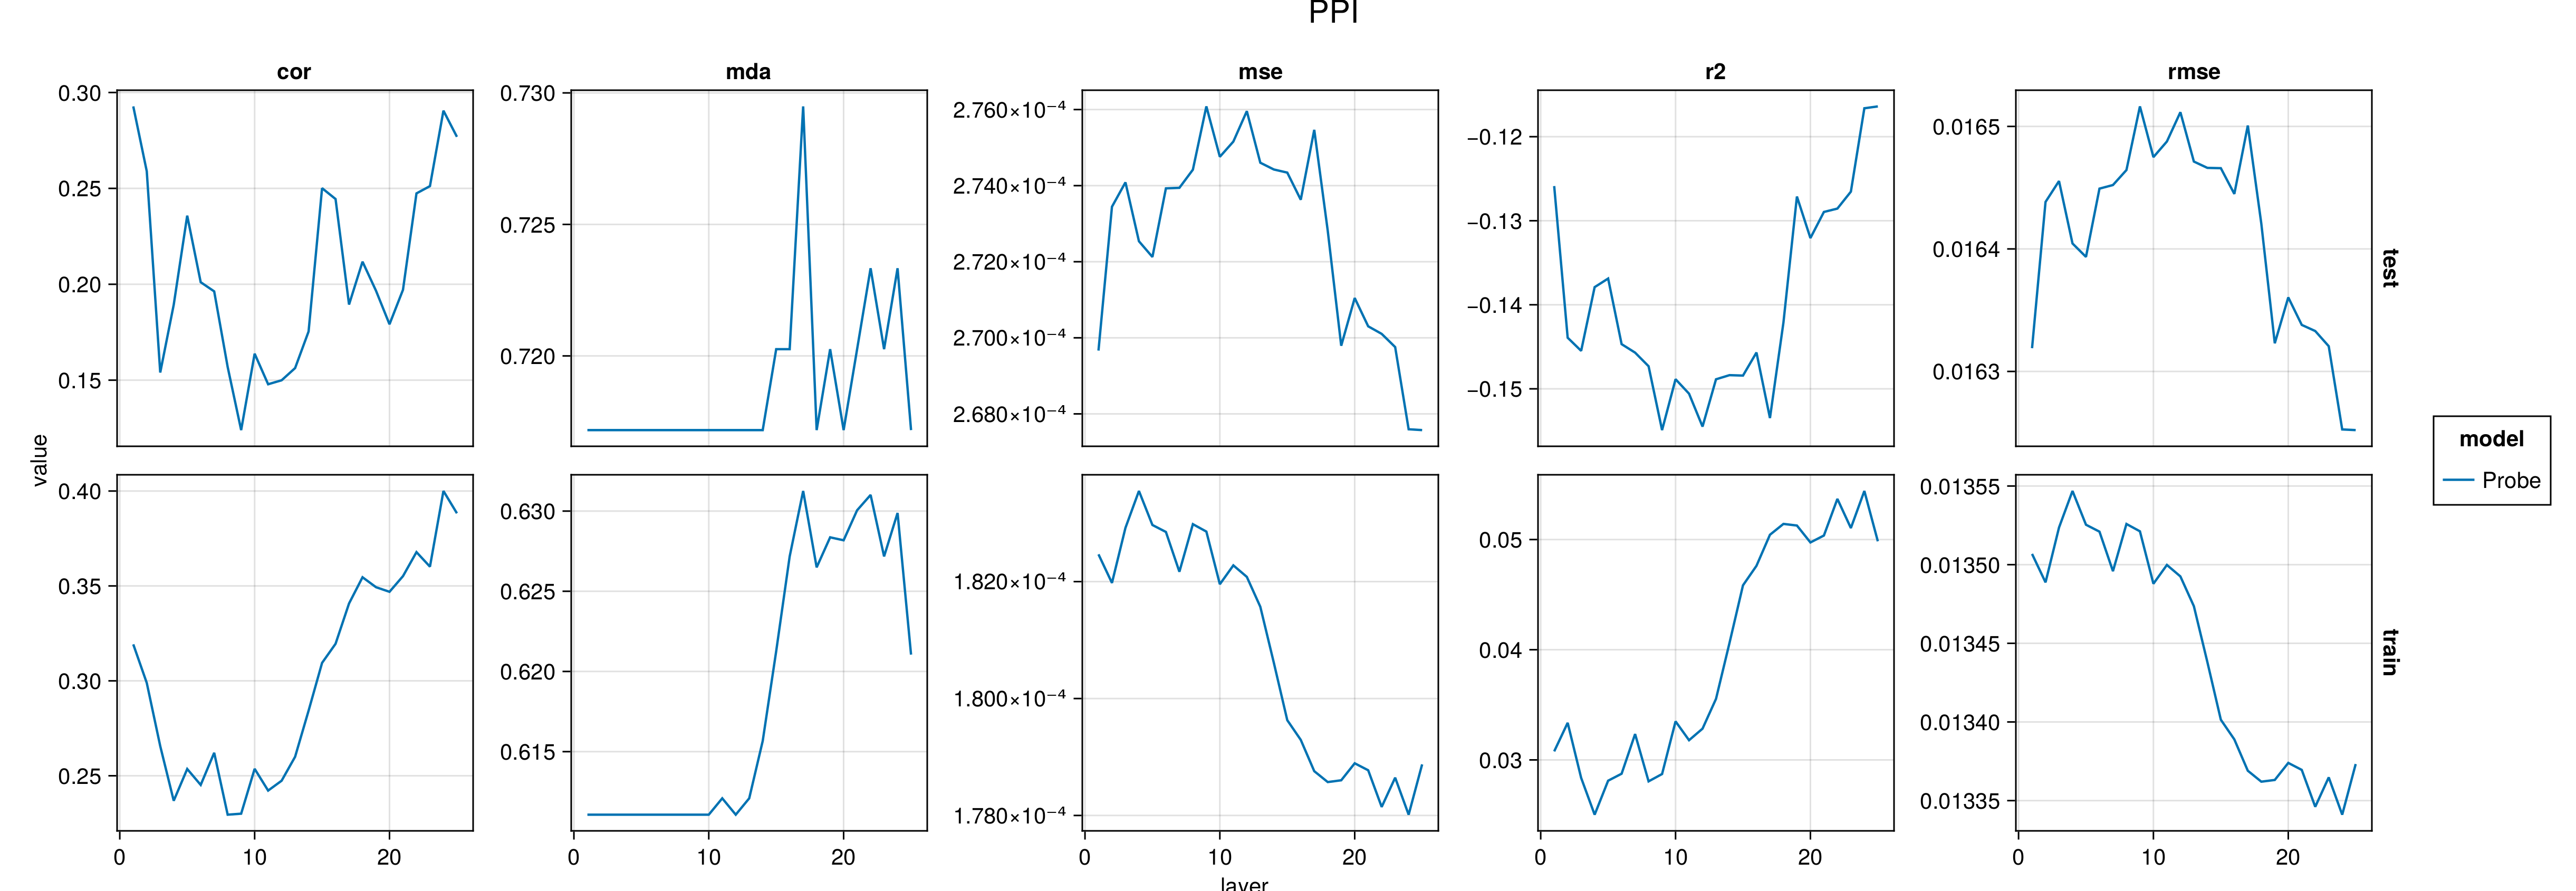
\includegraphics[width=1.0\textwidth]{results/figures/measures_probe_PPI (n_pc=128).png}

}

\caption{\label{fig-ppi}Average performance measures across folds plotted against model depth (number of layer) for the PPI for the train and test set.}

\end{figure*}%

% ---------- UST (1 Mo)  ----------

\begin{figure*}

\centering{

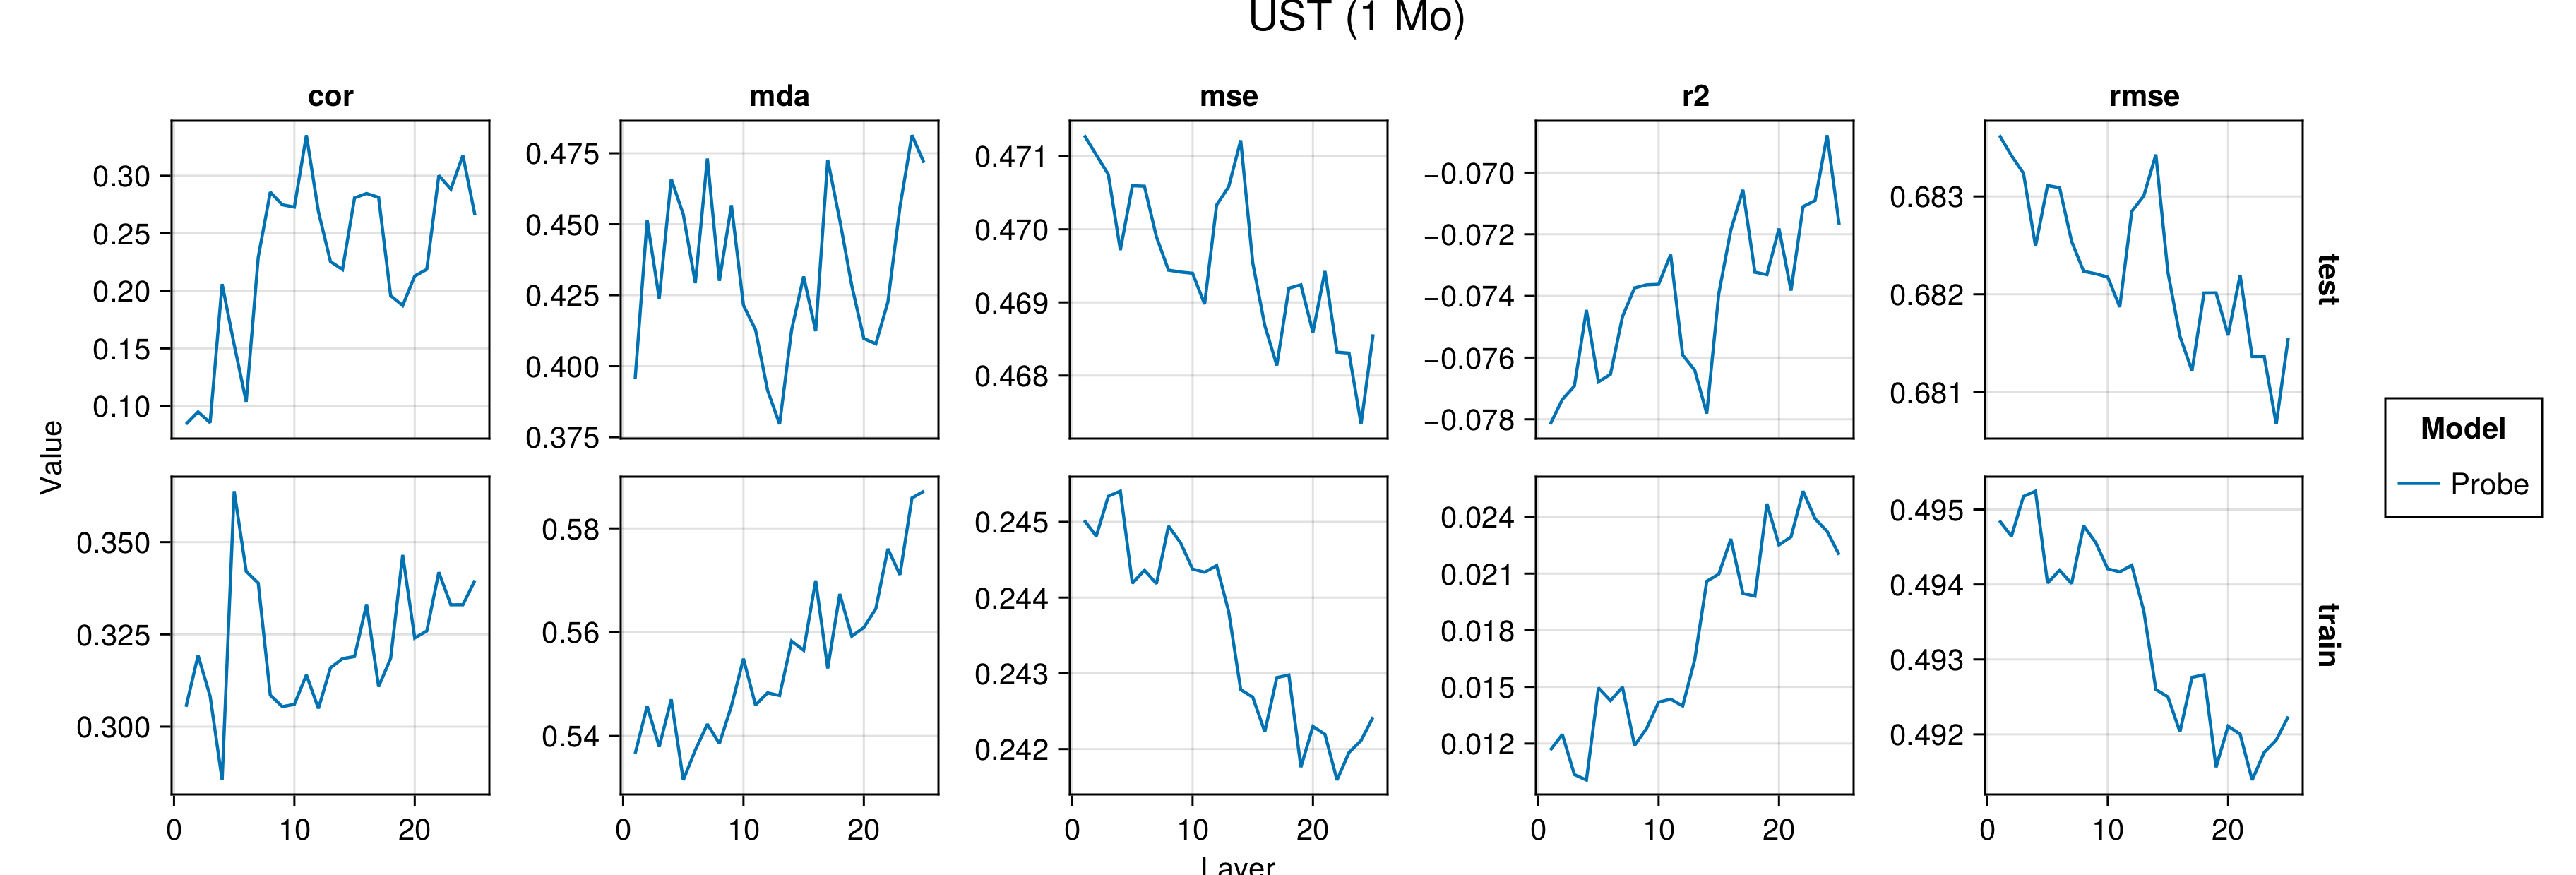
\includegraphics[width=1.0\textwidth]{results/figures/measures_probe_UST (1 Mo) (n_pc=128).png}

}

\caption{\label{fig-ust-1}Average performance measures across folds plotted against model depth (number of layer) for the UST (1 Mo) for the train and test set.}

\end{figure*}%

% ---------- UST (1 Yr)  ----------

\begin{figure*}

\centering{

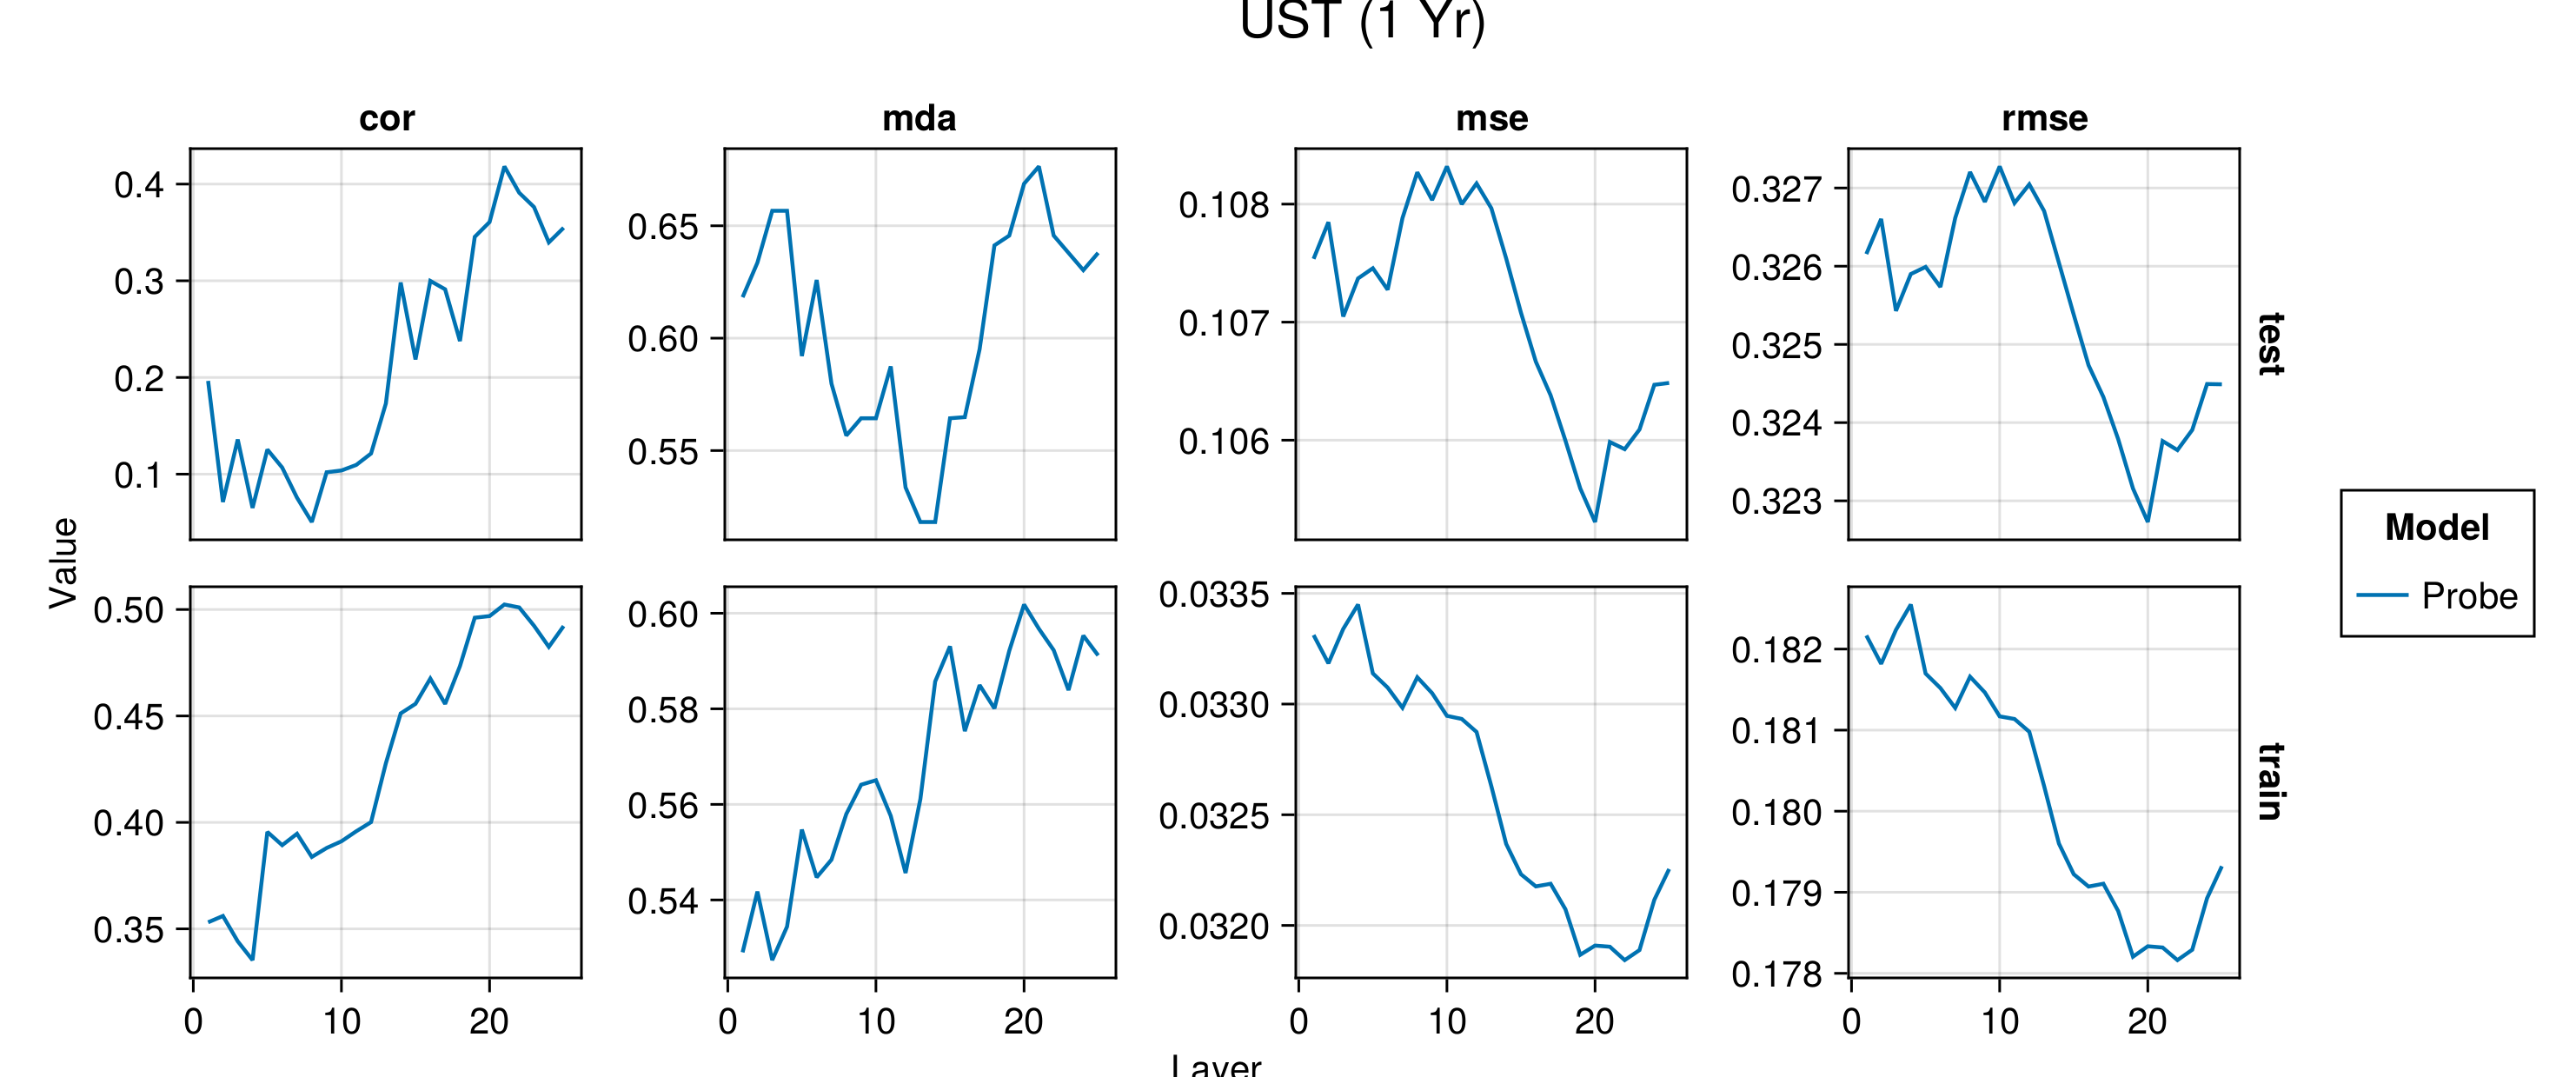
\includegraphics[width=1.0\textwidth]{results/figures/measures_probe_UST (1 Yr) (n_pc=128).png}

}

\caption{\label{fig-ust-1y}Average performance measures across folds plotted against model depth (number of layer) for the UST (1 Yr) for the train and test set.}

\end{figure*}%

% ---------- UST (10 Yr)  ----------

\begin{figure*}

\centering{

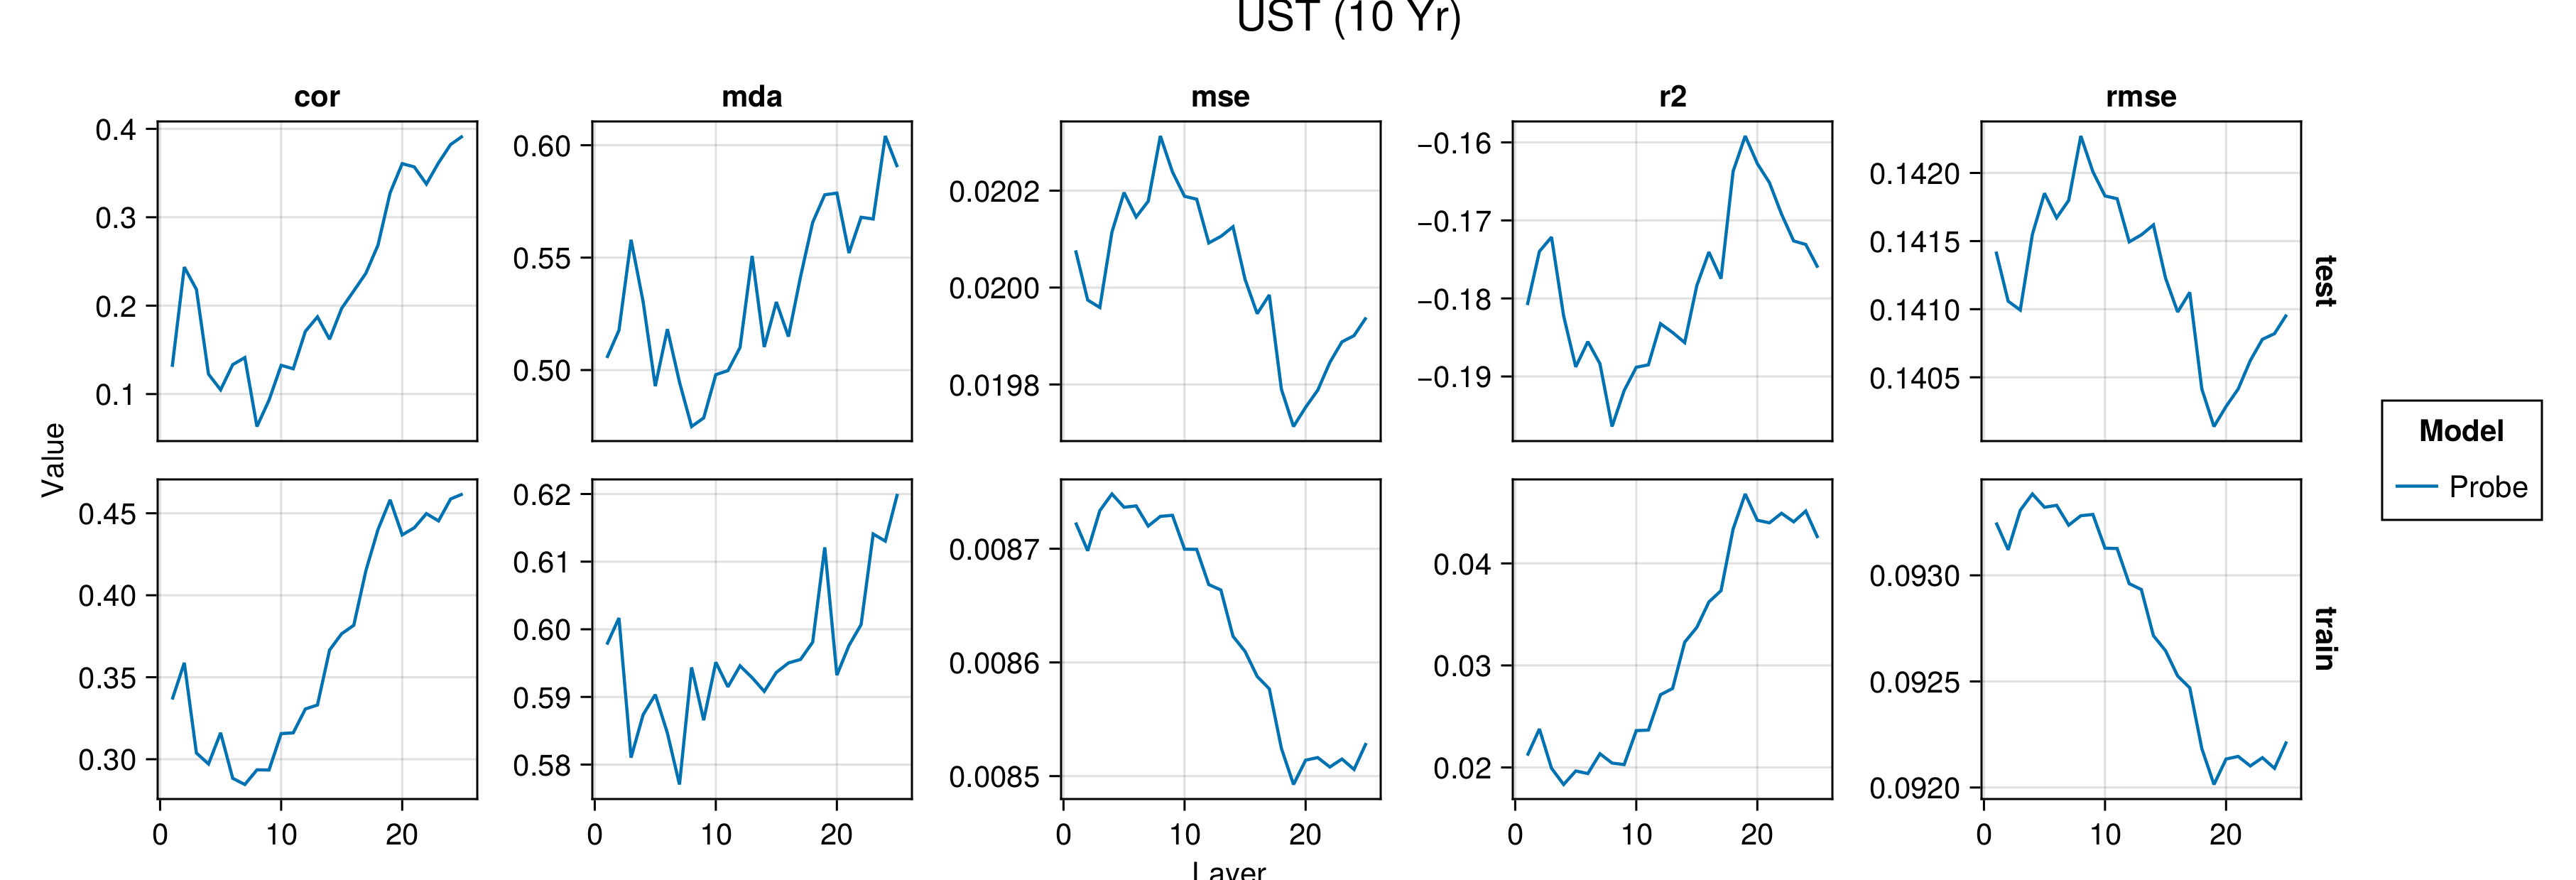
\includegraphics[width=1.0\textwidth]{results/figures/measures_probe_UST (10 Yr) (n_pc=128).png}

}

\caption{\label{fig-ust-10}Average performance measures across folds plotted against model depth (number of layer) for the UST (1 Yr) for the train and test set.}

\end{figure*}%

% -------- CPI benchmark --------

\begin{figure*}

\centering{

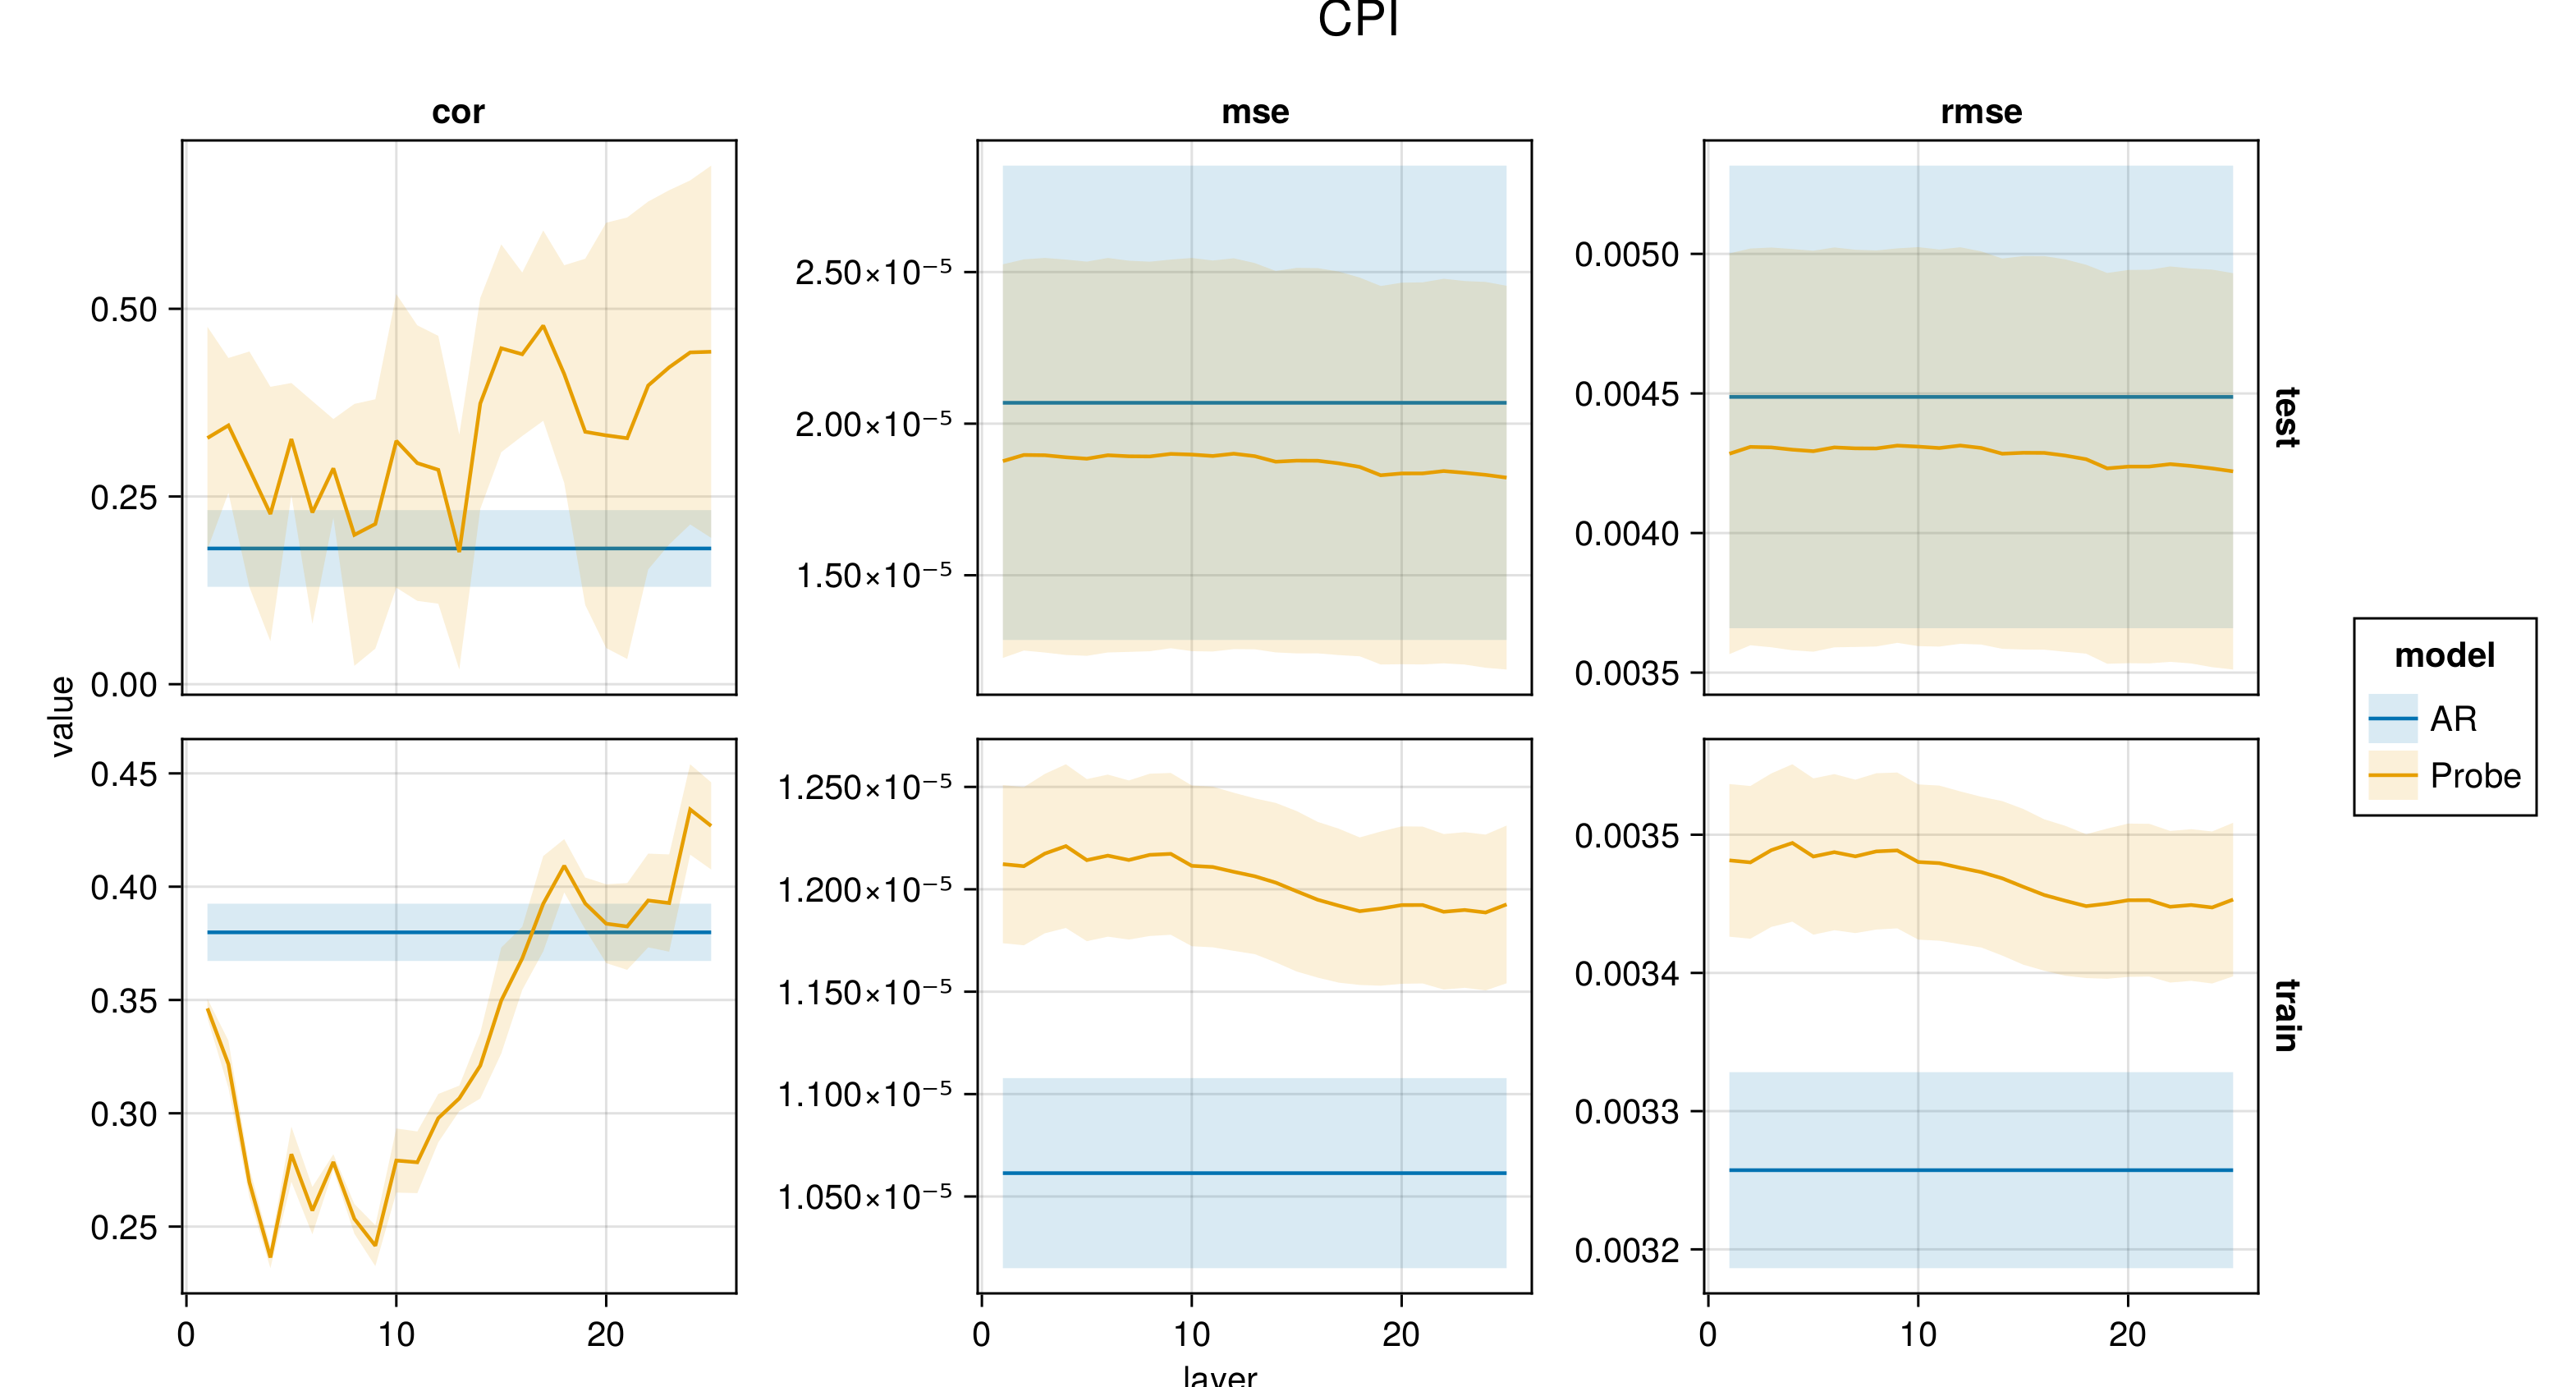
\includegraphics[width=1.0\textwidth]{results/figures/measures_CPI (n_pc=128).png}

}

\caption{\label{fig-cpi-b}Average performance measures across folds plotted against model depth (number of layer) for the CPI for the train and test set compared against the baseline autoregressive model. Shaded areas show the variation across folds.}

\end{figure*}%

% -------- PPI benchmark --------

\begin{figure*}

\centering{

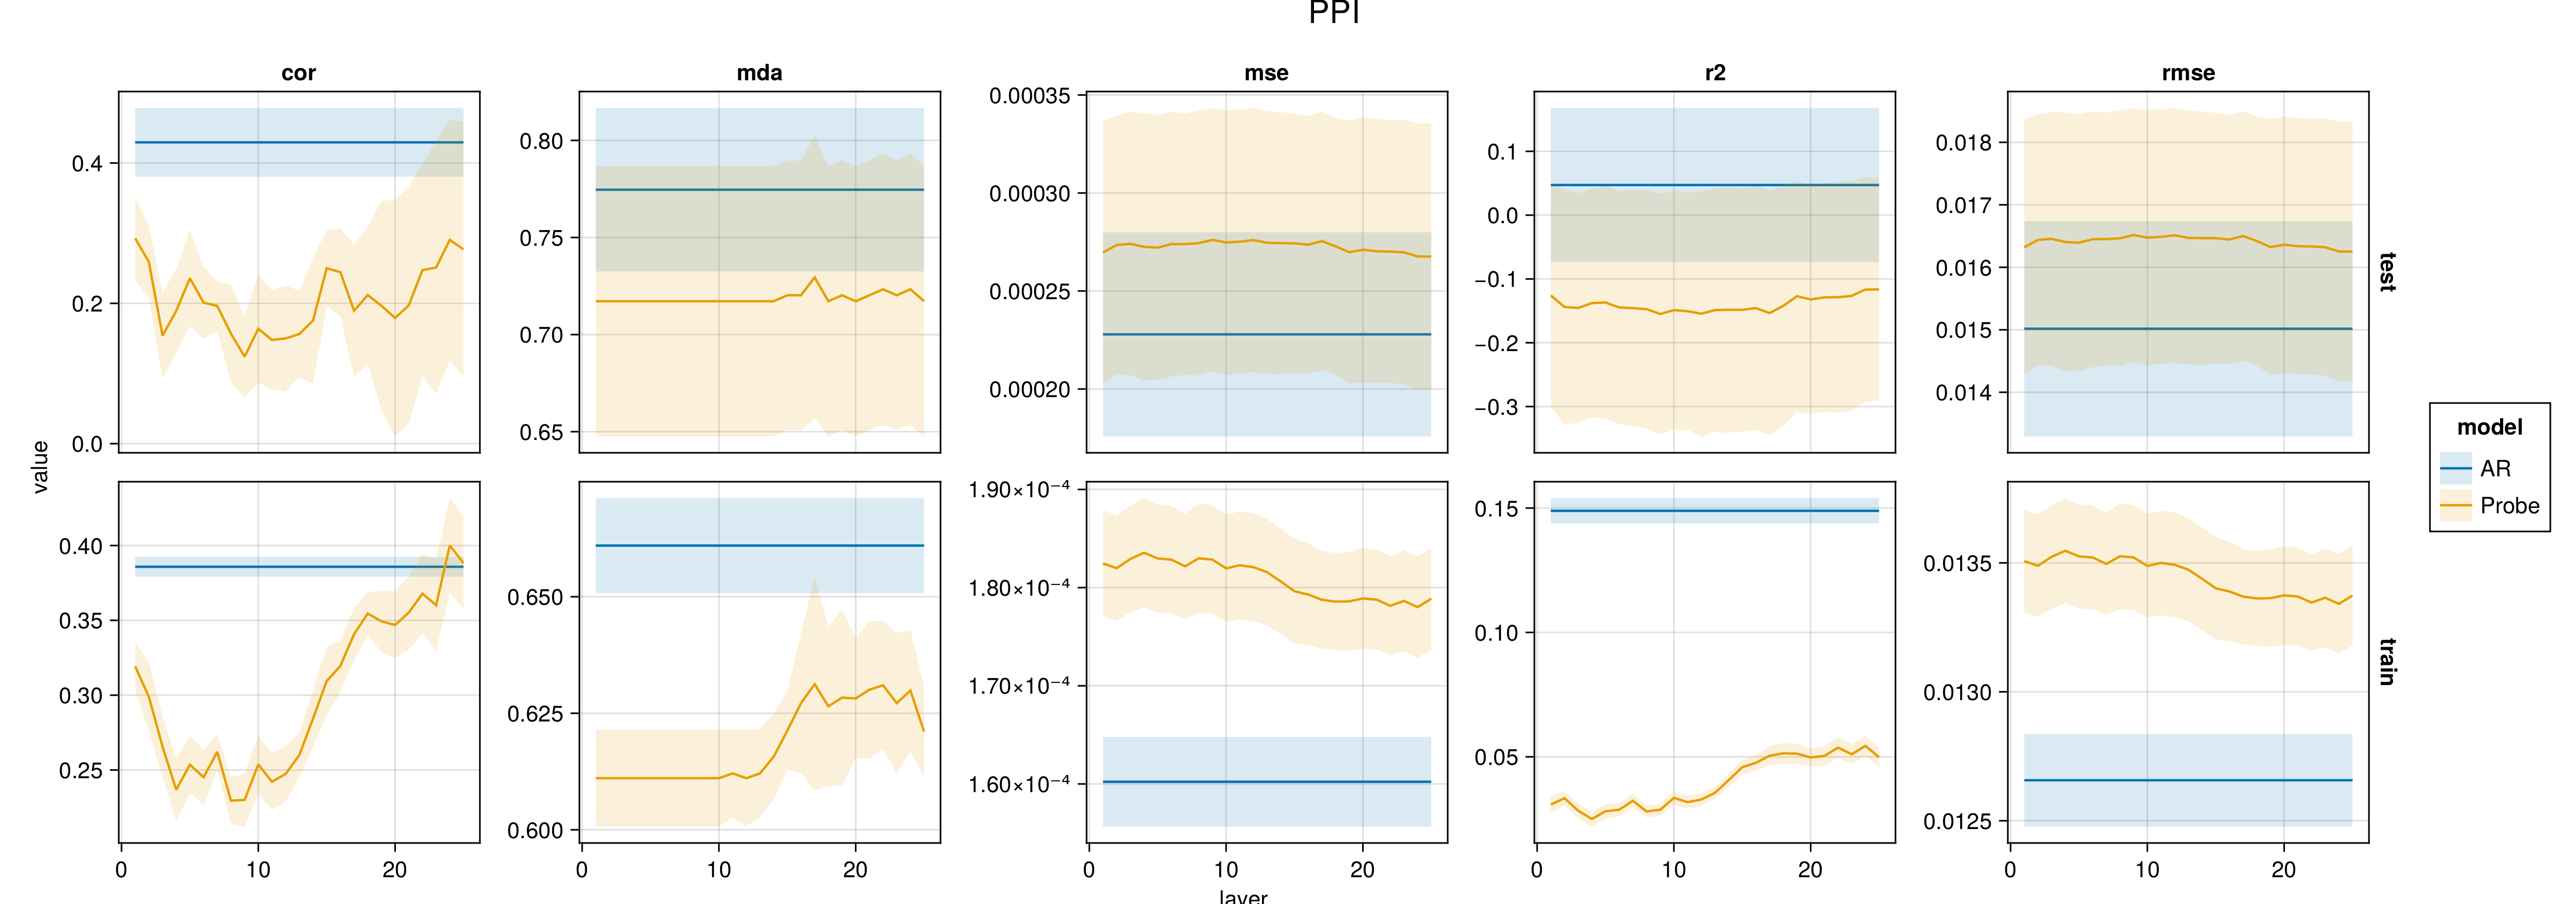
\includegraphics[width=1.0\textwidth]{results/figures/measures_PPI (n_pc=128).png}

}

\caption{\label{fig-ppi-b}Average performance measures across folds plotted against model depth (number of layer) for the PPI for the train and test set compared against the baseline autoregressive model. Shaded areas show the variation across folds.}

\end{figure*}%

% -------- UST (1 Mo) benchmark --------

\begin{figure*}

\centering{

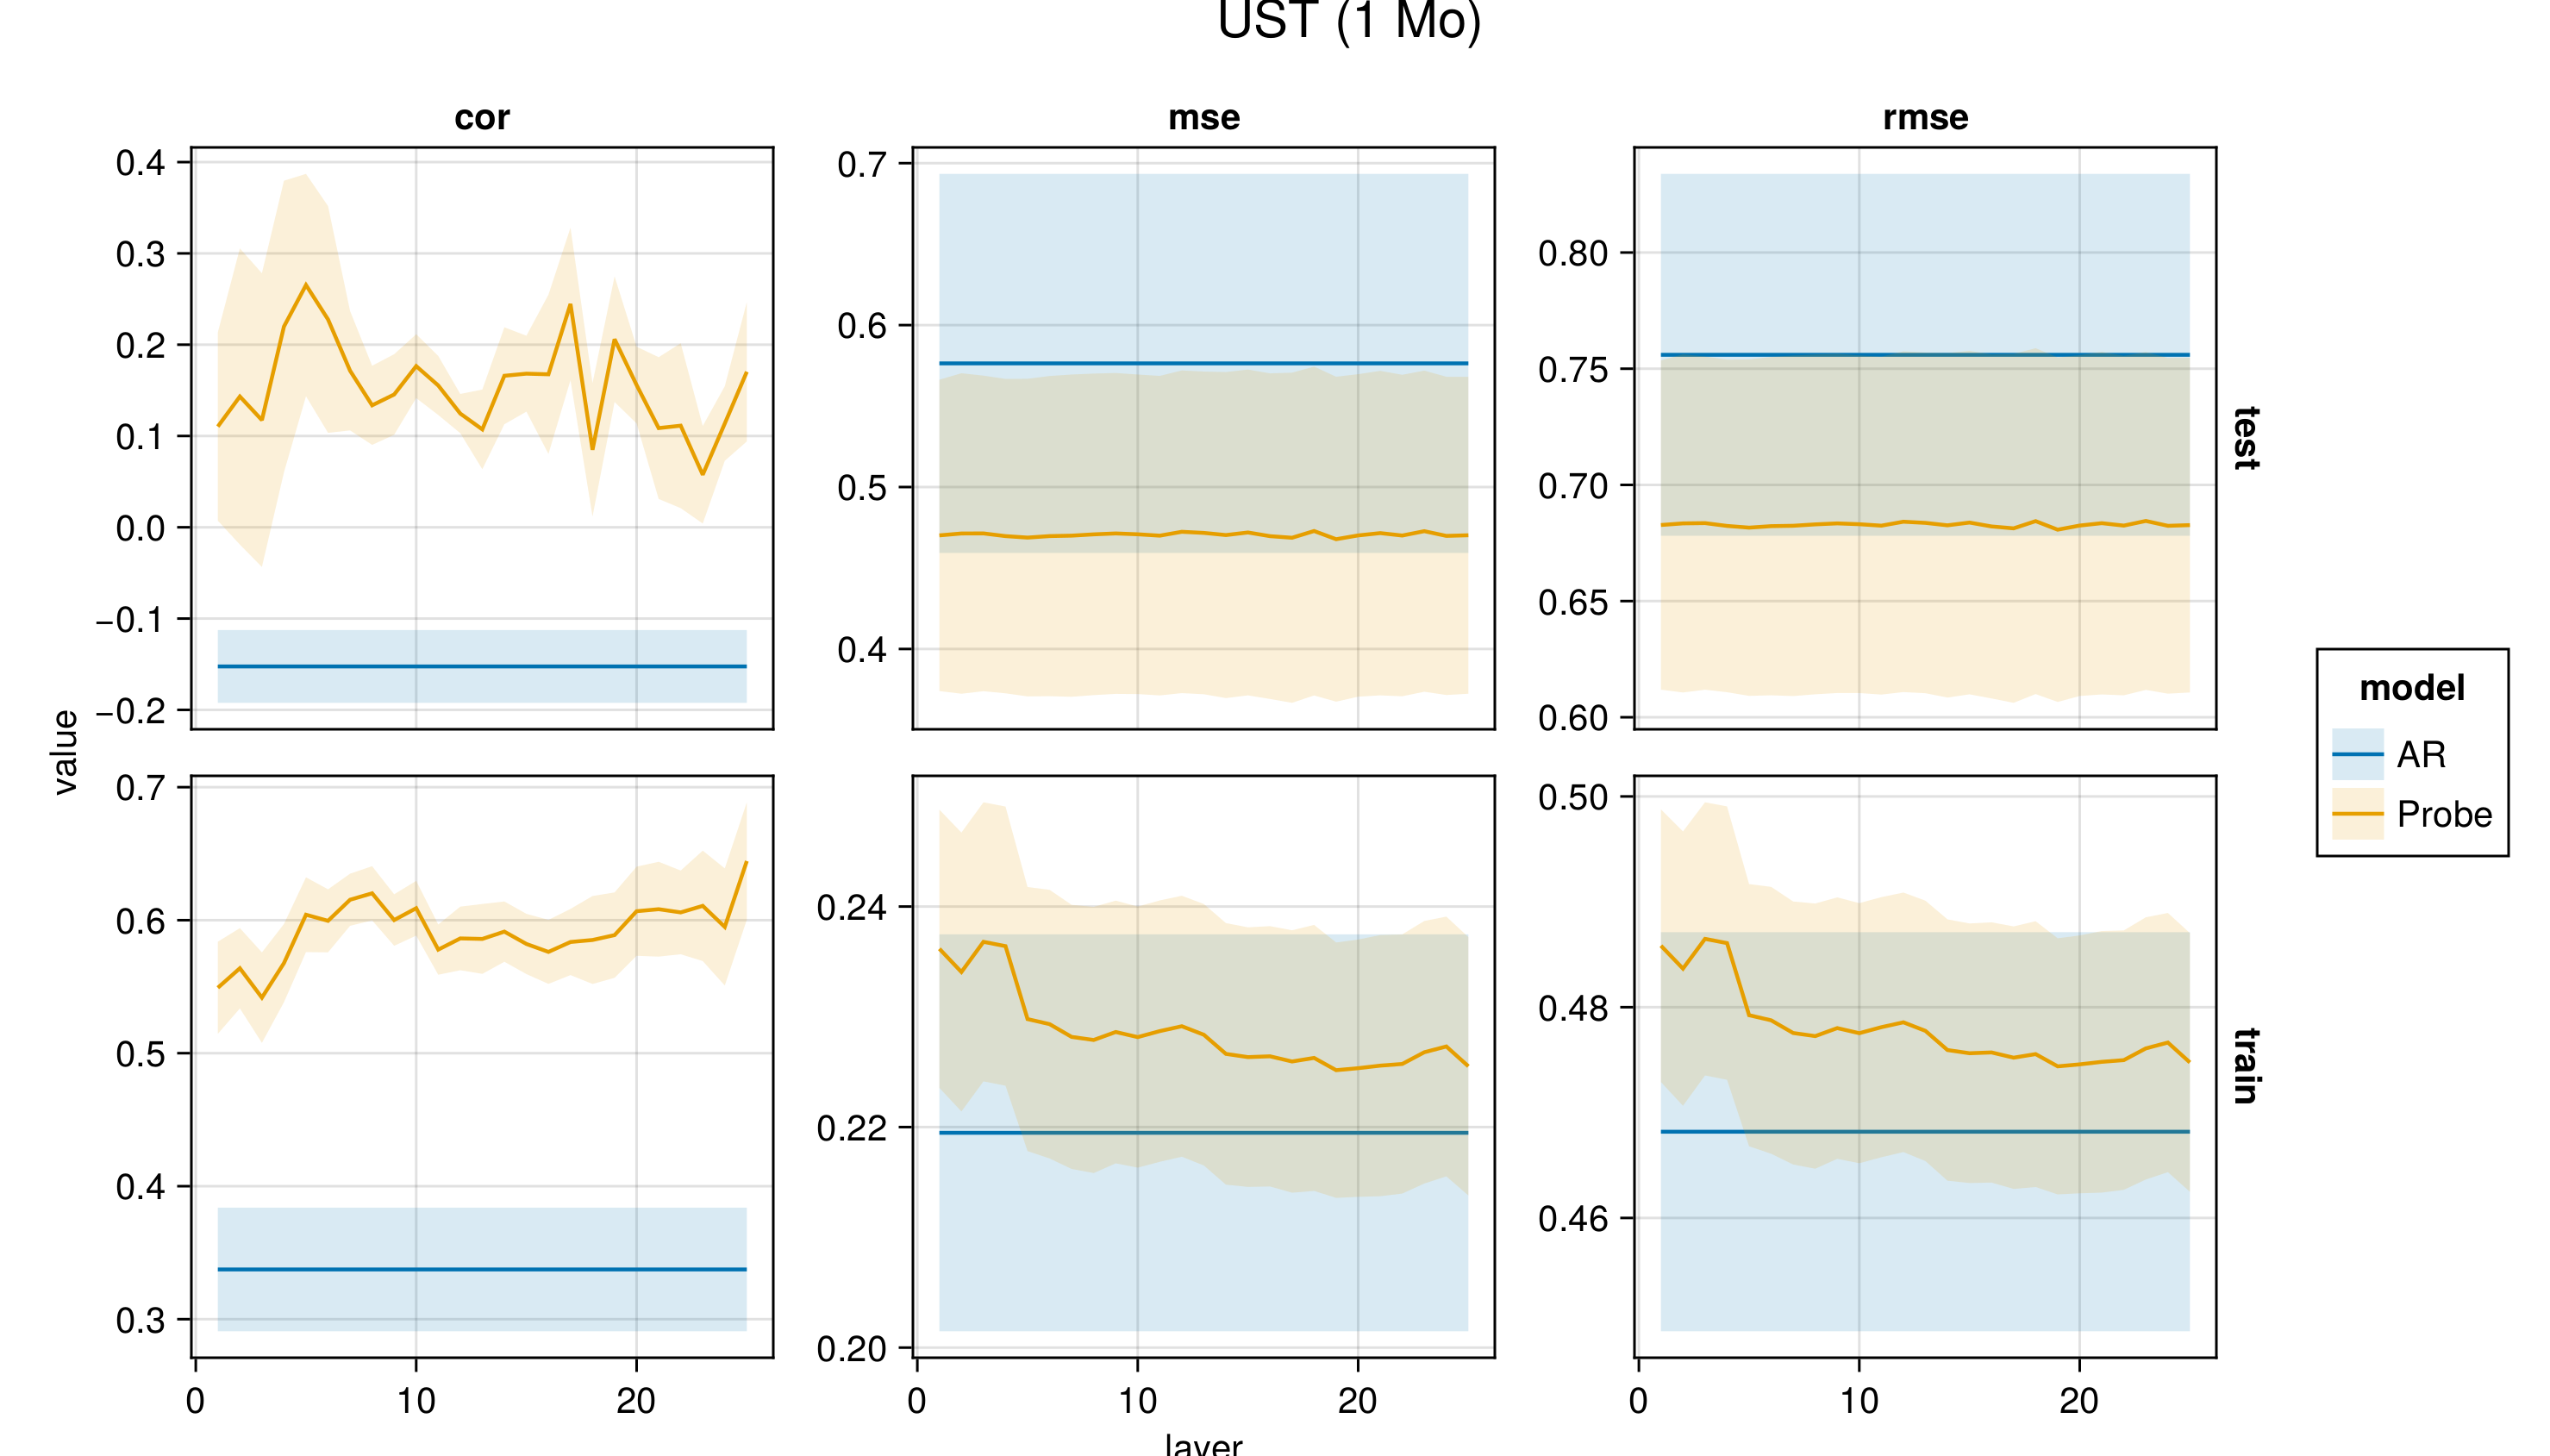
\includegraphics[width=1.0\textwidth]{results/figures/measures_UST (1 Mo).png}

}

\caption{\label{fig-ust-1-b}Average performance measures across folds plotted against model depth (number of layer) for the UST (1 Mo) for the train and test set compared against the baseline autoregressive model. Shaded areas show the variation across folds.}

\end{figure*}%

% -------- UST (1 Yr) benchmark --------

\begin{figure*}

\centering{

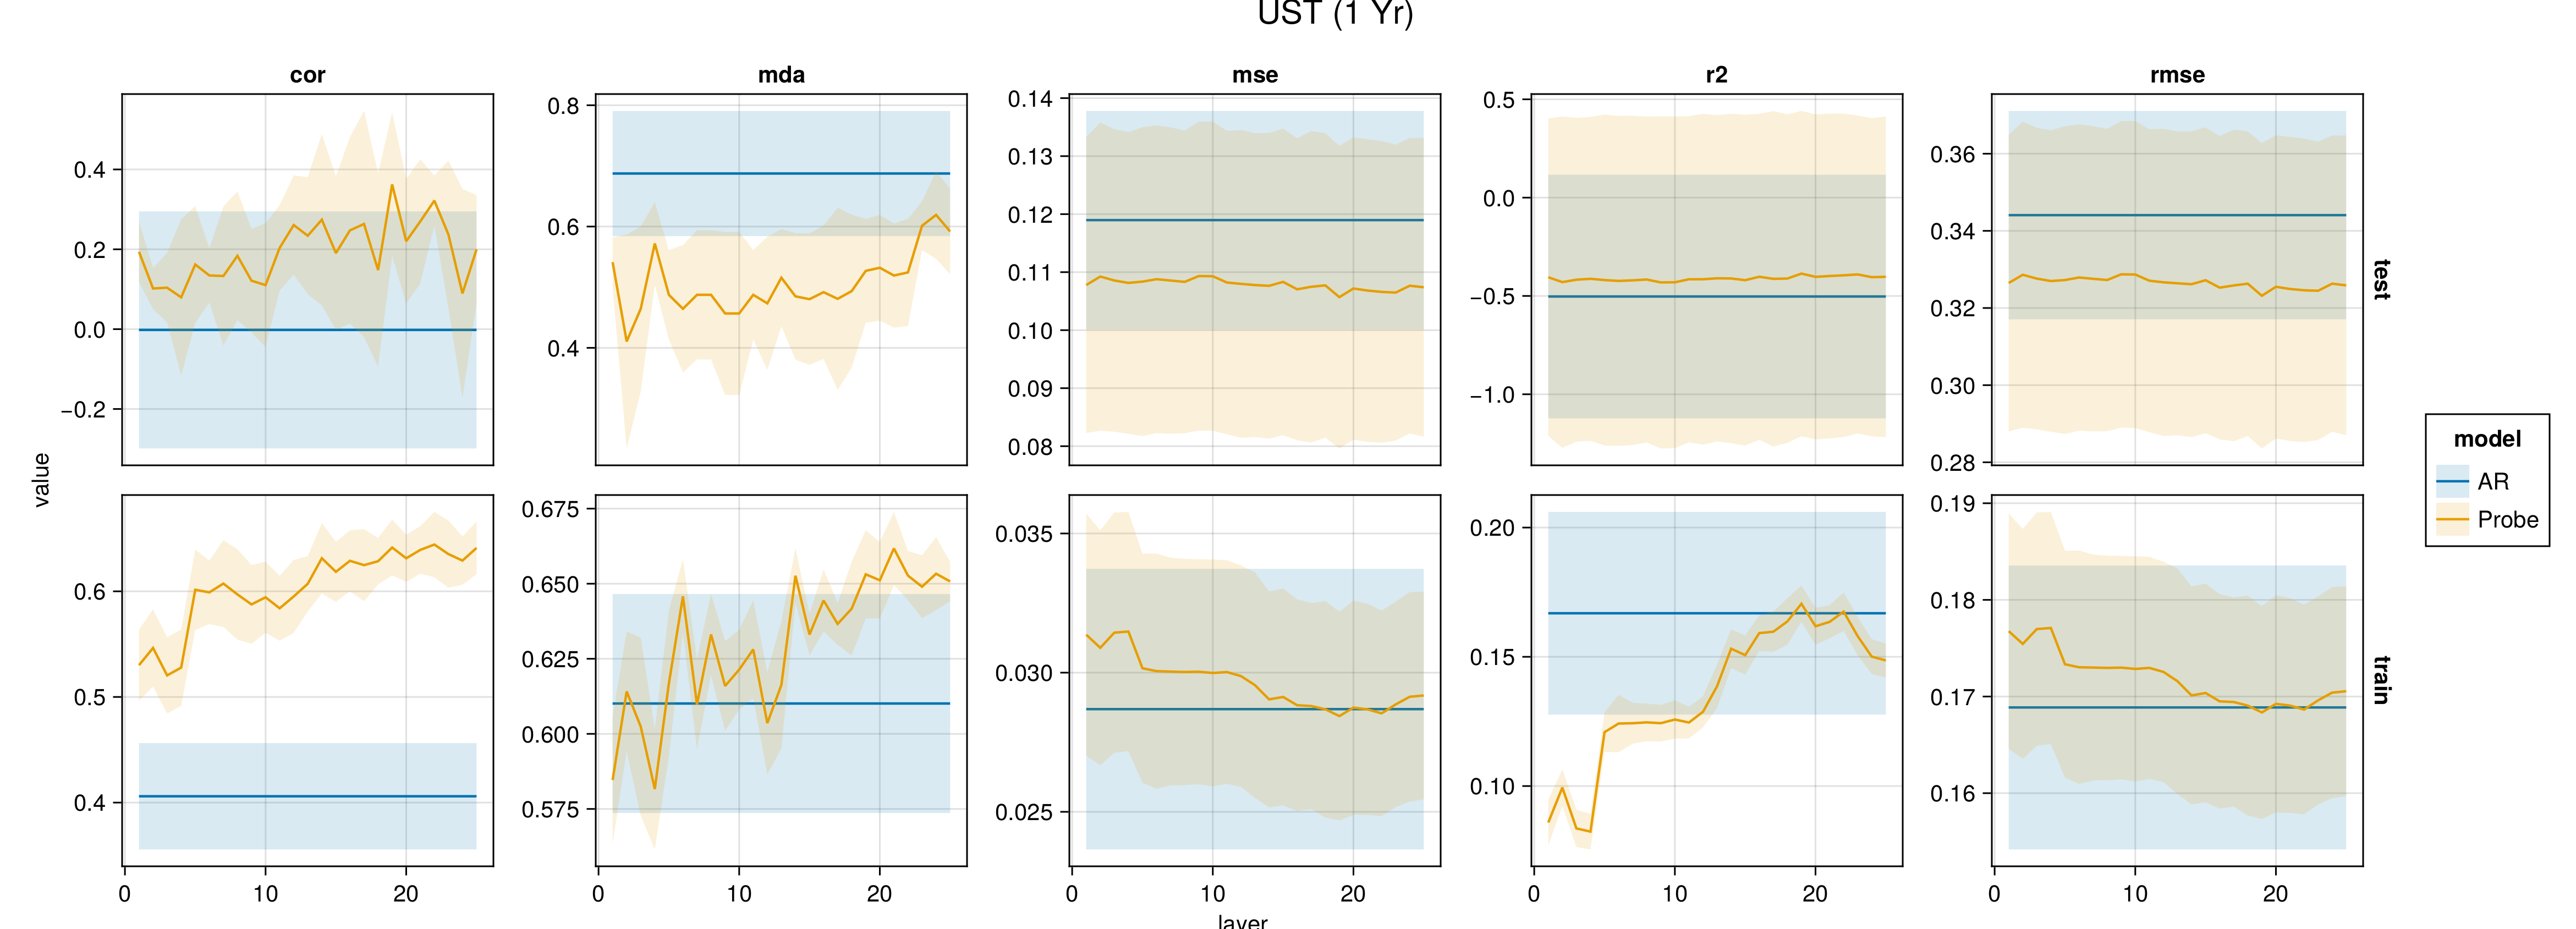
\includegraphics[width=1.0\textwidth]{results/figures/measures_UST (1 Yr).png}

}

\caption{\label{fig-ust-1y-b}Average performance measures across folds plotted against model depth (number of layer) for the UST (1 Yr) for the train and test set compared against the baseline autoregressive model. Shaded areas show the variation across folds.}

\end{figure*}%

% -------- UST (10 Yr) benchmark --------

\begin{figure*}

\centering{

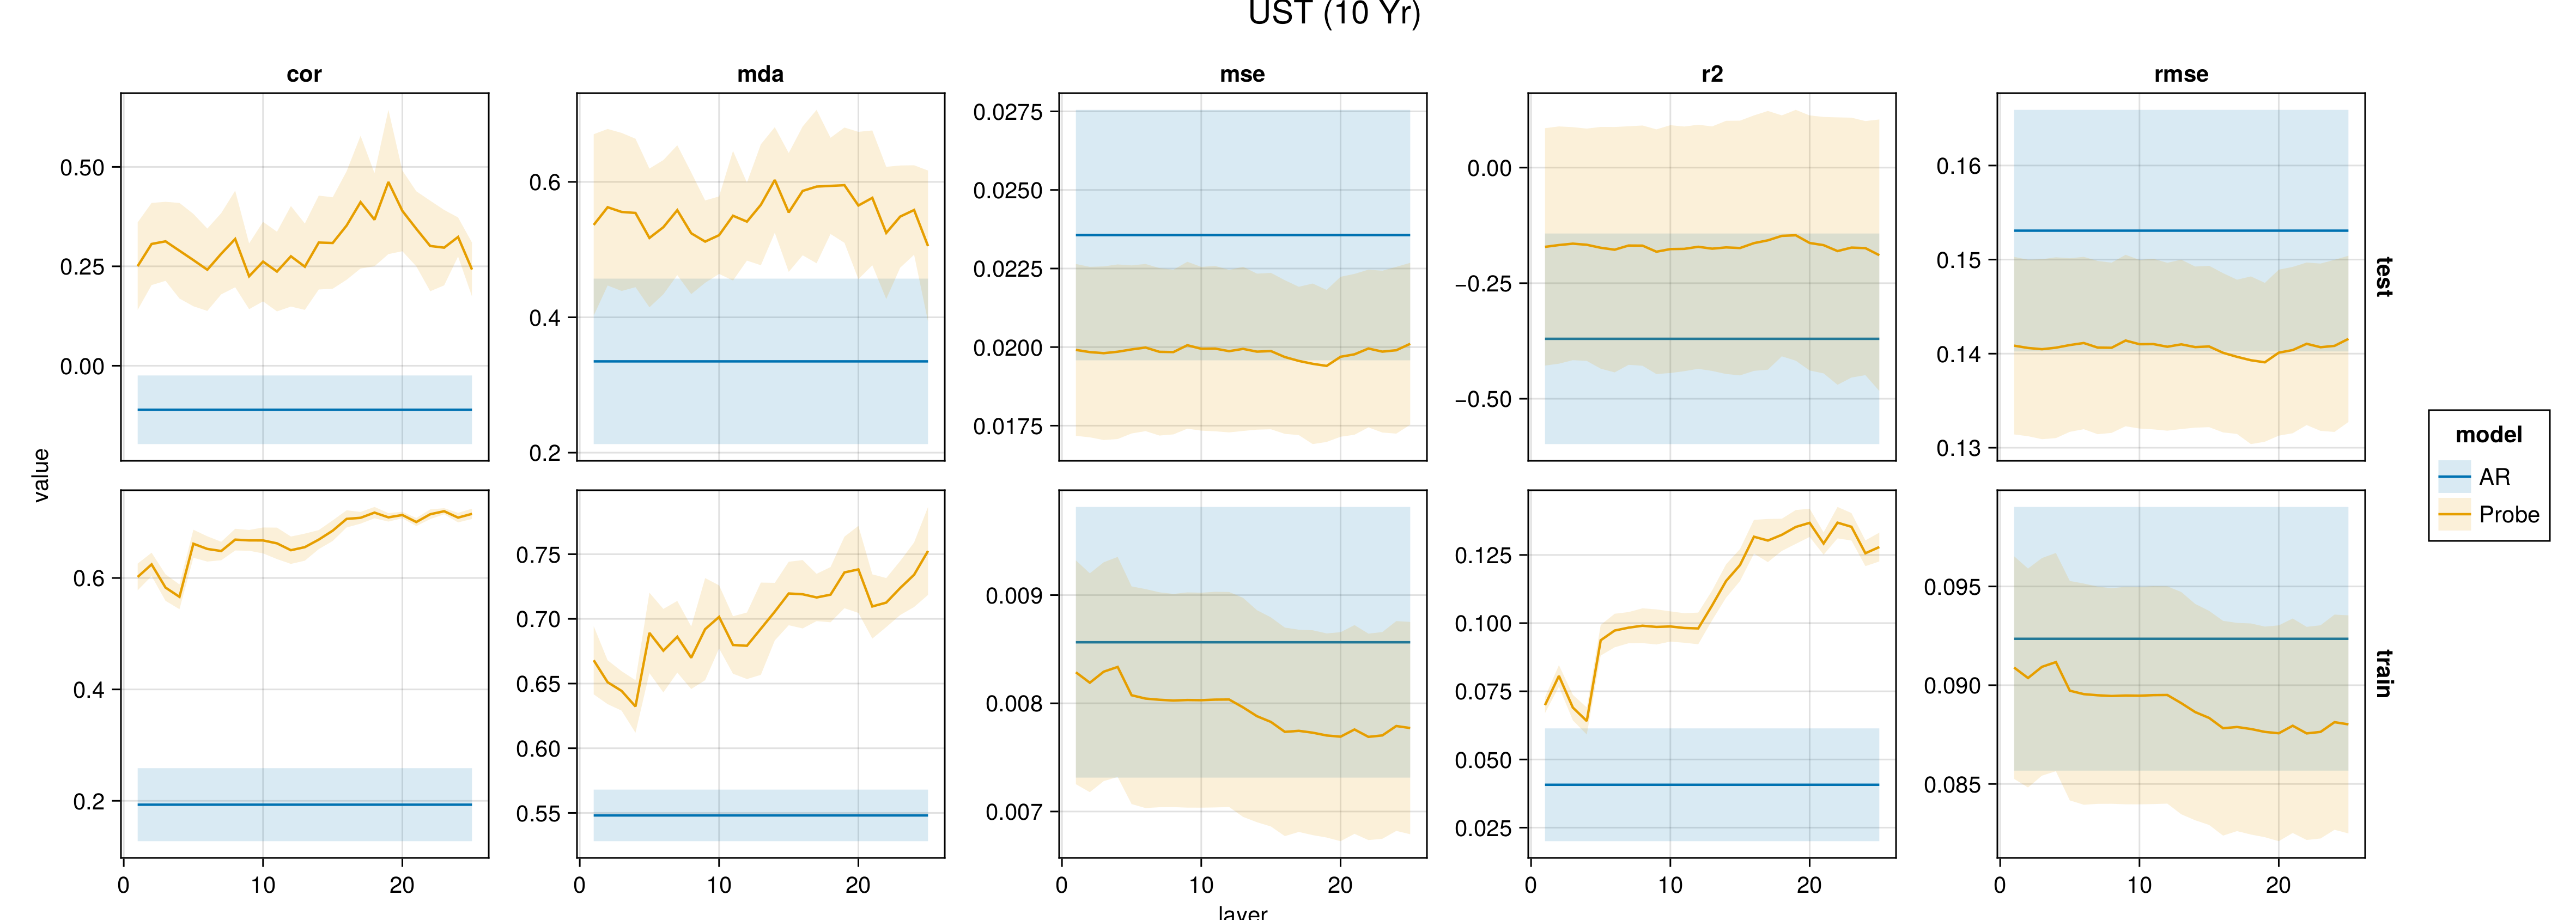
\includegraphics[width=1.0\textwidth]{results/figures/measures_UST (10 Yr).png}

}

\caption{\label{fig-ust-10-b}Average performance measures across folds plotted against model depth (number of layer) for the UST (10 Yr) for the train and test set compared against the baseline autoregressive model. Shaded areas show the variation across folds.}

\end{figure*}%

\section{Toward Parrot Tests}\label{appendix:parrot}

In our experiments from Section~\ref{ex-llm}, we considered the following hypothesis tests as a minimum viable testing framework to assess if our probe results (may) provide evidence for an actual `understanding' of key economic relationships learned purely from text:

\begin{proposition}[Parrot
Test]\protect\hypertarget{prp-line}{}\label{prp-line}

~

\begin{itemize}
\setlength\itemsep{1px}
\item
  \emph{H0 (Null)}: The probe never predicts values that are statistically significantly different from \(\mathbb{E}[f(\varepsilon)]\).
\item
  \emph{H1 (Stochastic Parrots)}: The probe predicts values that are statistically significantly different from \(\mathbb{E}[f(\varepsilon)]\) for sentences related to the outcome of interest \emph{and} those that are independent (i.e. sentences in all categories).
\item
  \emph{H2 (More than Mere Stochastic Parrots)}: The probe predicts values that are statistically significantly different from \(\mathbb{E} [f(\varepsilon)]\) for sentences that are related to the outcome variable (IP and DP), but not for sentences that are independent of the outcome (IB and DB).
\end{itemize}
\end{proposition}


To be clear, if in such a test we did find substantial evidence in favour of rejecting both \emph{HO} and \emph{H1}, this would not automatically imply that \emph{H2} is true. But to even continue investigating, if based on having learned meaningful representation the underlying LLM is more than just a parrot, it should be able to pass this simple test.

In this particular case, Figure~\ref{fig-attack} demonstrates that we find some evidence to reject \emph{H0} but not \emph{H1} for \emph{FOMC-RoBERTa}. The median linear probe predictions for sentences about inflation and deflation are indeed substantially higher and lower, respectively than for random noise. Unfortunately, the same is true for sentences about the inflation and deflation in the number of birds, albeit to a somewhat lower degree. This finding holds for both inflation indicators and to a lesser degree also for yields at different maturities, at least qualitatively.

We should note that the number of sentences in each category is very small here (10), so the results in Figure~\ref{fig-attack} cannot be used to establish statistical significance. That being said, even a handful of convincing counter-examples should be enough for us to seriously question the claim, that results from linear probes provide evidence in favor of real `understanding'. In fact, even a handful of sentences for which any human annotator would easily arrive at the conclusion of independence, a prediction by the probe in either direction casts doubt.

\section{Code}

All of the experiments were conducted on a MacBook Pro, 14-inch, 2023, with an Apple M2 Pro chip and 16GB of RAM. Forward passes through the FOMC-RoBERTa were run in parallel on 6 threads. All our code will be made publicly available. For the time being, an anonymized version of our code repository can be found here: \url{https://anonymous.4open.science/r/spurious_sentience/README.md}.